\section{Eclipse}
\subsection{Components}
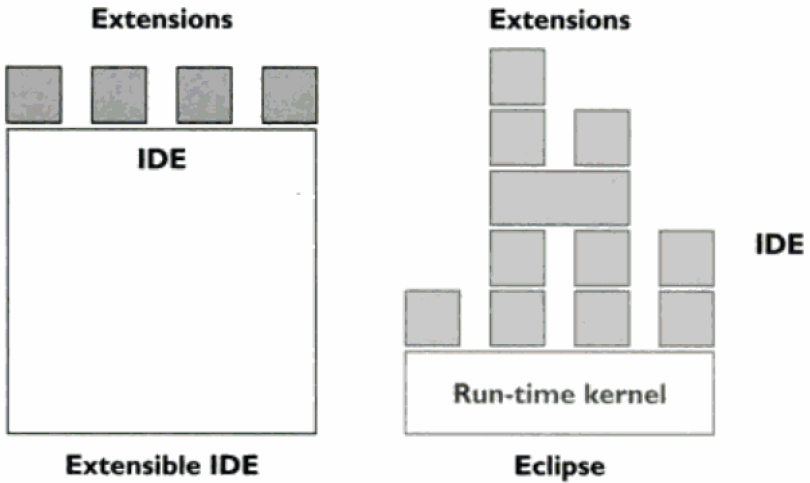
\includegraphics[width=0.7\linewidth]{./img/eclipse_components.png}
\subsubsection{SWT}
\begin{itemize}
    \item Native Widgets and mostly written in Java
    \item No performance implact form UI
    \item Provides basic Components
\end{itemize}
\subsubsection{JFace}
\begin{itemize}
    \item Builds on top of SWT 
    \item Actions 
    \item Menus 
    \item Dialogs 
    \item Wizards 
    \item Fonts 
\end{itemize}
\subsubsection{OSGi}
\begin{itemize}
    \item Specifies a component and service model for Java
    \item Components can be installed, started, stopped and uninstalled at runtime 
    \item Each bundle gets its own classloader
    \item Bundles define dependencies and export some of their packages
\end{itemize}
\textbf{Bundles:}
\begin{itemize}
    \item Eclipse Plugins are OSGi Bundles
    \item Packaged as JARs
    \item MANIFEST.MF contains the bundle metadata
\end{itemize}
\textbf{Services:}
\begin{itemize}
    \item Connect Bundles
    \item Service is a POJO and can be registered at a Service Registry at bundle start
    \item Eclipse does not use OSGi services but Extensions and Extension Points
\end{itemize}

\subsubsection{Extension Points}
\begin{itemize}
    \item Collect contributions to the plug-in offering the Extension Point 
    \item Each plug-in contributes to at least one extension point
    \item EP and Extensions are not part of the Manifest but separate XML files
\end{itemize}
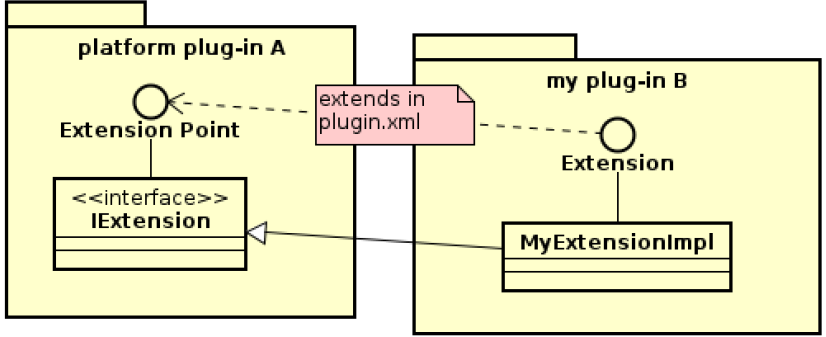
\includegraphics[width=0.7\linewidth]{./img/ep.png}

\subsection{Eclipse Plug-ins}
\begin{itemize}
    \item Add new Actions, Editors, Views, Perspectives, Preferences
    \item Each one gets its own class loader
    \item Can only access specified dependencies
    \item Has three interesting files
    \begin{itemize}
        \item Manifest
        \item plugin.xml: wires up the Extension
        \item Class that imlements the Extension
    \end{itemize}
\end{itemize}
\textbf{Eclipse Platform}
\begin{itemize}
    \item Manages Plugins
    \item Discover installed plug-ins
    \item builds the extension registry
    \item connects extesions and EP
    \item Only activates plug-ins when needed
\end{itemize}

\subsection{GoF Design Patterns in Eclipse}
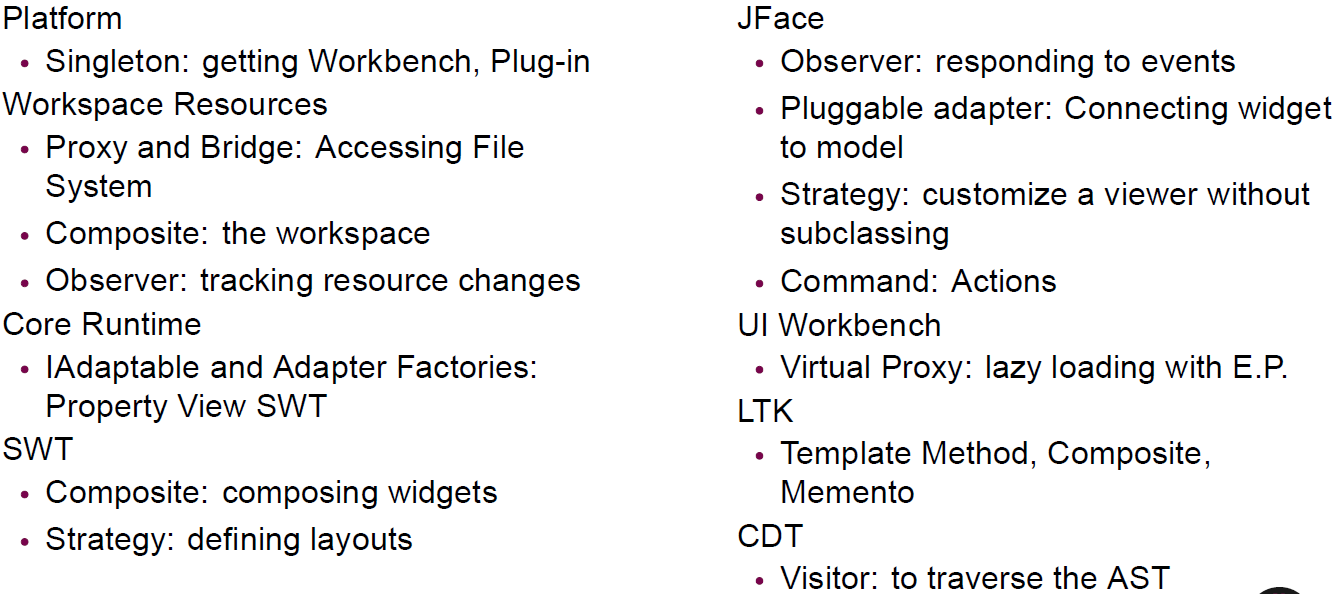
\includegraphics[width=\linewidth]{./img/eclipse_gof.png}

\subsection{Refactoring Language Toolkit (LTK)}
\begin{itemize}
    \item Language neutral API for refactorings
    \item Classes for constructing refactoring UI (common L\&F for wizards)
    \item Refactoring wizard with diff preview
    \item Classes for modelling resource changes
    \item Refactoring participant functionality
\end{itemize}
\subsubsection{Refactoring Lifecycle Overview}
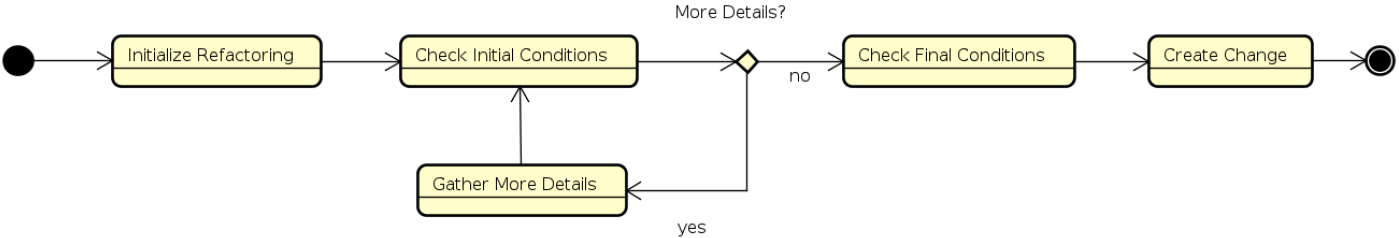
\includegraphics[width=\linewidth]{./img/refactoring_lc.png}

\subsubsection{Refactoring Participants}
\begin{itemize}
    \item Can participate in the condition checking and change creation of a refactoring processor
    \item Refactorings that change multiple files may have an impact on other tools
\end{itemize}

